\documentclass[12pt, twoside]{article}
\usepackage[letterpaper, margin=1in, headsep=0.5in]{geometry}
\usepackage[english]{babel}
\usepackage[utf8]{inputenc}
\usepackage{amsmath}
\usepackage{amsfonts}
\usepackage{amssymb}
\usepackage{tikz}
\usepackage{yhmath}
%\usetikzlibrary{quotes, angles}

\usepackage{graphicx}
\usepackage{enumitem}
\usepackage{multicol}

\usepackage{fancyhdr}
\pagestyle{fancy}
\fancyhf{}
\renewcommand{\headrulewidth}{0pt} % disable the underline of the header

\fancyhead[RE]{\thepage}
\fancyhead[RO]{\thepage \\ Name: \hspace{3cm}}
\fancyhead[L]{BECA / Dr. Huson / 10th Grade Geometry\\* 3 February 2020}

\begin{document}
\subsubsection*{8.5 Do Now: Volumes \& solid geometry}
 \begin{enumerate}

  \item Find the area of a semi-circle with diameter of 9 centimeters.
   \begin{flushright}
    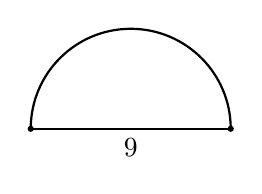
\begin{tikzpicture}[scale=.635]
      %\draw [help lines] (-5,-1) grid (5,4);
      \draw [thick] (-2,0)-- (2,0);
      %\draw [thick, ->] (0,-2.2)--(0,10.4) node [left] {$y$};
      \draw [thick] (2,0) arc (0:180:2);
      \draw [fill] (-2,0) circle [radius=0.05];
      \draw [fill] (2,0) circle [radius=0.05];
      \node at (0,0)[below]{9};
    \end{tikzpicture}
  \end{flushright}

  \item Given circle $O$ with radius $OB=12$ cm.
    \begin{multicols}{2}
    \raggedcolumns
    \begin{enumerate}
      \item Find the circumference of circle $O$. \vspace{1.7cm}
      \item Find the area of the circle.  \vspace{2cm}
      \item A regular heptagon (7 sides) is inscribed in the circle, with $A$ and $B$ two of its vertices. \\[0.25cm]
      Find the area of the sector $AOB$. \vspace{1.5cm}
    \end{enumerate}
      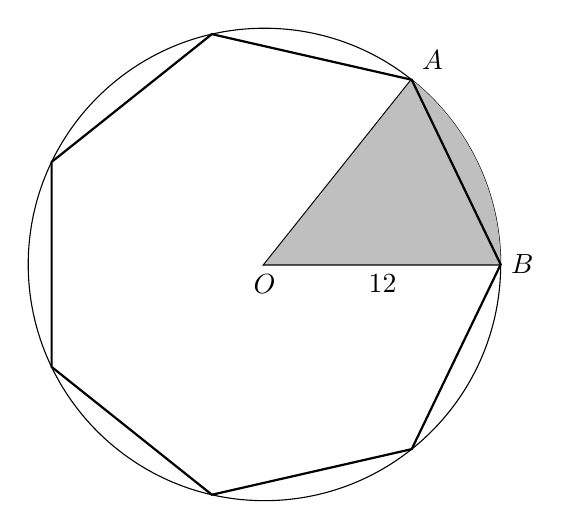
\begin{tikzpicture}[scale=1]
        \draw (0,0) circle[radius=3];
        \draw [thick]
        (0:3) node[right] {$B$}--
        (0,0) node[below] {$O$}--
        (1*360/7:3) node[above right] {$A$};
        \fill [lightgray]
        (0,0)--(0:3) arc (0:1*360/7:3)--(0,0);
        \draw (1.5,0) node[below] {$12$};
        \draw [thick] (0:3)--(1*360/7:3)--(2*1*360/7:3)--(3*1*360/7:3)--
        (4*1*360/7:3)--(5*1*360/7:3)--(6*1*360/7:3)--cycle;
      \end{tikzpicture}
    \end{multicols}  \vspace{3cm}

  \item Find the volume of a pyramid ($V=\frac{1}{3}Bh$) having a height of 9 meters and with a square base having side lengths of 14 meters. Express your result to the \emph{nearest cubic meter}. \vspace{5cm}

\newpage
\subsubsection*{The equation of a circle}

  \item A circle centered at the origin includes the point $(8,6)$, as shown below.
  \begin{multicols}{2}
    \raggedcolumns
    \begin{enumerate}
      \item Find the radius of the circle. \vspace{2.7cm}
      \item Name another point on the circle as an ordered pair.
    \end{enumerate}
      \begin{tikzpicture}[scale=.7]
        \draw (0,0) circle[radius=5];
        \draw [thick]
        (0:4) node[below] {$(8,0)$}--
        (0,0) node[below] {$(0,0)$}--
        (4,3) node[above right] {$(8,6)$}--cycle;
        \draw [dashed] (0,0)--(5,0);
        \draw (3.5,0)--(3.5,0.5)--(4,0.5);
      \end{tikzpicture}
  \end{multicols}

  \item What is the equation of a circle with center $(1,-5)$ and radius $r=3$. Use the equation $(x-a)^2+(y-b)^2=r^2$. \vspace{1.5cm}
  
\subsubsection*{Applying density ratios}
  \item A large block of stone has a volume of 12 cubic feet. The density of stone is 140 pounds per cubic feet. Find the weight of the block.  \vspace{3cm}
  \item A tank of heating oil holds 250 gallons. Find the cost to completely fill the tank if heating oil costs \$3.45 per gallon. \vspace{3cm}


\end{enumerate}
\end{document}
